\section{Autotuning and Distributed Computing}
\label{sec:autotuningCloud}

This implementation and study was developed shortly after our initial work on
autotuning for NVCC parameters. We identified limitations of the OpenTuner
framework in relation to parallel and distributed execution of measurements
and decided that it would be an interesting pursuit to attempt to extend
the framework so that it could leverage public cloud services.

This section describes the methodology and protocol we implemented as
extensions to the OpenTuner framework, distributing and parallelizing the
exploration of optimization spaces by combining results obtained from virtual
machines in the Google Compute Engine (GCE).  A local machine (LM) runs the
main OpenTuner application. Several virtual machines (VMs) run measurement
modules and provide results when requested. This distributed approach performs
a more cost efficient exploration of the search space in comparison to the
sequential execution.

In a progression of
papers~\cite{gupta2012exploring,gupta2014evaluating,gupta2013the}, Gupta
\emph{et al.} provide experimental evaluations of the application of cloud
computing to high performance computing, describing which kind of applications
has the greatest potential to benefit from cloud computing.  Their work
highlights small and medium scale projects as the main beneficiaries of cloud
computing resources. This is a strong motivation for performing autotuning
runs using those resources.

We faced problems related to initial implementation choices. The number of
external IPs that the Google Compute Engine provides limited our possibilities
for experiments and impacted the validation of this approach. Despite that, we
still believe that these extensions are worth pursuing and hope to validate it
with more time-consuming applications and more virtual machines.

\subsection{Parallel and Distributed Programming in OpenTuner}
\label{subsec:parallel}
\todo[inline,author=Pedro,color=cyan]{Discuss the difficulties and
explain why they motivated the new Julia code.}

\subsection{Methodology and Protocol}
\label{sec:ext}

The methodology and protocol we propose follow the client-server model,
distributing measurements of program configurations between a group of VMs
running \emph{MeasurementServer}s in the cloud. The servers wait for
measurement requests from a client, and maintain copies of the program to be
autotuned and the user-defined function that measures configurations.

The machine running the autotuner runs a \emph{MeasurementClient}, an
extension of the native \emph{MeasurementDriver}, that instead of compiling and
running result requests locally, uses an interface to route requests to VMs and
then saves the results to the local database.

Figures~\ref{fig:high-level} and~\ref{fig:low-level} present an overview of the
architecture of the extension.  Figure~\ref{fig:high-level} presents the
architecture of an OpenTuner application running the measurement client and
communicating with the measurement servers.  Green boxes in the figure
represent OpenTuner modules that are not modified, and blue boxes represent new
or modified modules.

Figure~\ref{fig:low-level} shows, on a lower level of abstraction, the
interactions between the measurement client and servers. The client requests
results from the server through a wrapper of the GCE Python API.  The GCE
interface also encapsulates the application protocol used in the client-server
communication.

\begin{figure}[htpb]
    \centering
    \begin{minipage}{.45\textwidth}
        \centering
        \includegraphics[scale=.64]{high-level-implementation}
        \caption{A high-level view of the architecture.}
        \label{fig:high-level}
    \end{minipage}%
    \hfill
    \begin{minipage}{.45\textwidth}
        \centering
        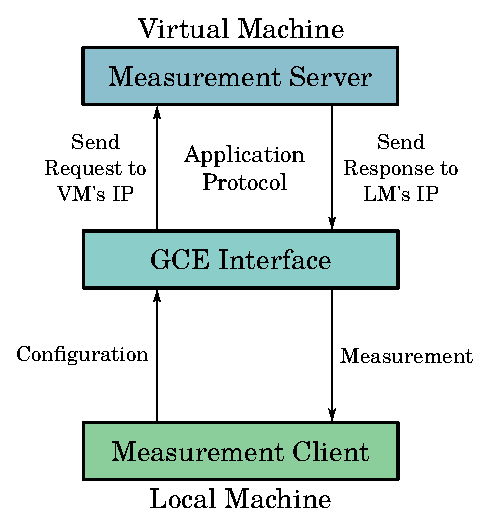
\includegraphics[scale=.64]{low-level-implementation}
        \caption{A lower-level view of the architecture.}
        \label{fig:low-level}
    \end{minipage}%
    \label{fig:archs}
\end{figure}

\subsubsection{Measurement Server and Client}
\label{sec:server-client}

OpenTuner controls the execution flow of an application with the
\texttt{\footnotesize main} function of the \emph{TuningRunMain} class. This
function initializes the database and the search and measurement modules. It
then calls the \texttt{\footnotesize main} function of the search driver, which
runs the main loop of the application.  The search driver generates
configurations to be tested and saves them to the database. It then calls the
\texttt{\footnotesize process\_all} function of the measurement driver and
blocks until the function returns.

The \texttt{\footnotesize process\_all} function calls the
\texttt{\footnotesize run\_desired\_results} function, which is able to run
compilations in parallel but only sequential measurements.  The modified
\emph{MeasurementDriver} initializes the GCE interface during its own
initialization. During execution the overridden \texttt{\footnotesize
process\_all} and \texttt{\footnotesize run\_desired\_results} functions route
the result requests to the VMs using the \emph{GCEInterface}.  An instance of
the \emph{MeasurementServer} runs in every VM. The server waits for TCP
connections from a single client.

\subsubsection{GCE Interface}
\label{sec:gce}

The interactions between the local \emph{MeasurementClient} and the VMs'
\emph{MeasurementServer}s are mediated by the \emph{GCEInterface}, a wrapper of
the GCE Python API.  The interface starts and configures VMs storing each
measurement server's IP.

The interface enables the \emph{MeasurementClient} to request results from the
servers without knowledge of the application protocol. Running our
client-server methodology in another cloud environment would require a new
interface that manages VMs in this environment, but no modifications to the
server or client would be needed.

\subsubsection{Application Protocol}
\label{sec:app}

This section describes the text-based application protocol used in the
client-server communications mediated by the \emph{GCEInterface}. The user's
OpenTuner application must be a git project available via
\texttt{\footnotesize{HTTP}}. The application will be cloned to the VM by the
server using the \texttt{\footnotesize CLONE} message.  The application's
\texttt{\footnotesize run} method will be used to obtain autotuning results
requested by the client.

\paragraph{Messages}
\begin{table}[htpb]
    \centering
    \scriptsize
    \begin{tabular}{@{}p{2.1cm}p{4cm}p{6cm}@{}}
        \toprule
        {\bf Command} & {\bf Function} & {\bf Message} \\ \midrule
        {\scriptsize \bf START} &
        {\scriptsize Sets the server's status to AVAILABLE} &
        {\scriptsize \tt \lq{}START\rq{}} \\
        \addlinespace{}
        {\scriptsize \bf STOP} &
        {\scriptsize Sets the server's status to STOPPED} &
        {\scriptsize \tt \lq{}STOP\rq{}} \\
        \addlinespace{}
        {\scriptsize \bf STATUS} &
        {\scriptsize Requests the server current status} &
        {\scriptsize \tt \lq{}STATUS\rq{}} \\
        \addlinespace{}
        {\scriptsize \bf DISCONNECT} &
        {\scriptsize Disconnects from the server} &
        {\scriptsize \tt \lq{}DISCONNECT\rq{}} \\
        \addlinespace{}
        {\scriptsize \bf SHUTDOWN} &
        {\scriptsize Disconnects and shuts the server down} &
        {\scriptsize \tt \lq{}SHUTDOWN\rq{}} \\
        \addlinespace{}
        {\scriptsize \bf CLONE} &
        {\scriptsize Clones a git repository to the virtual machine} &
        {\scriptsize \tt \lq{}CLONE REPO\_URL DIST\_DIR\rq{}} \\
        \addlinespace{}
        {\scriptsize \bf LOAD} &
        {\scriptsize Imports the user's MeasurementInterface into the server} &
        {\scriptsize \tt \lq{}LOAD TUNER\_PATH INTERFACE\_NAME\rq{}} \\
        \addlinespace{}
        {\scriptsize \bf MEASURE} &
        {\scriptsize Computes the measurement for a given configuration} &
        {\scriptsize \tt \lq{}MEASURE CONFIG INPUT LIMIT\rq{}} \\
        \addlinespace{}
        {\scriptsize \bf GET} &
        {\scriptsize Requests a configuration's result} &
        {\scriptsize \tt \lq{}GET RESULT\_ID\rq{}} \\ \bottomrule
    \end{tabular}
    \caption{Server messages.}
    \label{tab:protocol-messages}
\end{table}

Table~\ref{tab:protocol-messages} shows all the messages in the protocol, a
brief description of their meaning and their string format. The client must
send a \texttt{\footnotesize MEASURE} message for each configuration that is
measured. The server returns a unique ID that is used to retrieve the results
when they are ready. This is done by sending a \texttt{\footnotesize GET}
message.

\paragraph{Server Responses}

The server responds to each request with a message template and trailing,
message-specific parameters. Responses always start with the correspondent
command name and end with a newline character.  Each response contains the
current server status (\texttt{\footnotesize SERVER\_STATUS}) and error code of
the command (\texttt{\footnotesize ERROR\_STATUS}).  The optional argument list
(\texttt{\footnotesize [ARGS..]}) contains the measurement result, for example,
in the case of a successful \texttt{\footnotesize GET} response.
Figure~\ref{fig:response-template} shows the format of a server response.

\begin{figure}[htpb]
    \centering
    \footnotesize
    \begin{tabular}{@{}c@{}}
        \toprule
        {\tt \lq{}COMMAND ERROR\_STATUS SERVER\_STATUS [ARGS..] [MESSAGE]\rq{}} \\ \bottomrule
    \end{tabular}
    \caption{The format of a server response.}
    \label{fig:response-template}
\end{figure}

All the code implemented for the proposed methodology and protocol is publicly
available at \path{github.com/phrb/measurement-server},
\path{github.com/phrb/gce_interface} and
\path{github.com/phrb/measurement_client} under the GNU General Public License.

\subsection{Result Normalization}
\label{sec:norm}

The VM instances available in public cloud computing services vary in multiple
aspects, such as available memory, number of processing cores and disk size.
When autotuning a program for a certain target machine, using instances hosted
at a public cloud, it is typical that the target architecture will differ from
the VMs'. Depending on the configuration of the cloud application the instances
could also have different architectures.

To effectively leverage cloud computing resources for autotuning, a
normalization technique must be devised that enables the results found in the
VMs to be valid for the target machine.  We present four approaches to this
problem. The best approach for each problem domain must be experimentally
determined, and could be a combination of the approaches described here.

\paragraph{Autotune Performance Models}
Another autotuner could be implemented to optimize parameters of a simple
performance model, that would associate a configuration's measurement and the
VM that produced it with a conversion function that transposes
performance results to the target architecture.

\paragraph{Ensembles of Virtual Machines}
The cloud application could be composed of VMs with different architectures.
The final performance measurement for a configuration would be built from some
combination of the results obtained in these different VMs.

\paragraph{Architecture Simulators}
The target machine could be modeled by an architecture simulator such as
\emph{zsim}~\cite{sanchez2013zsim}, a simulator for multi-core architectures.
Using a simulator would solve the normalization problem but introduce other
problems, such as the simulator's accuracy and performance.

\paragraph{Autotune in the Cloud}
Finally, the normalization problem could be sidestepped, at least in initial
stages of research, by running the servers and clients in the cloud using the
same kind of VM.

\subsection{Experiments}
\label{sec:exp}

This section describes the Travelling Salesperson Problem (TSP), the Google
Compute Engine's virtual machines and project settings used to evaluate the
efficacy of the proposed methodology and protocol.  The performances of
the autotuner for the TSP were measured in 8 different
experimental settings. Each tuning run lasted 15 minutes, used 2 or 4
virtual machines, and was repeated 4 times.  We also varied the number of
result requests that each virtual machine in a tuning run processed, namely 1,
4, 8 or 16 requests per machine.
The LM used had an 8-core Intel Xeon E3 and 32GB of RAM.

\subsubsection{Using the Google Compute Engine}

All virtual machines used in the experiments had a single vCPU and 3.75GB of
RAM (Google Compute Engine machine type \texttt{\footnotesize n1-standard-1}).
All experiments were performed with machines from the \texttt{\footnotesize
us-central1-f} zone. We built a virtual machine image with the latest stable
Debian distribution and all dependencies installed, speeding up the virtual
machines' initialization time.

\subsubsection{Travelling Salesperson Problem}

The instances of the TSP used in the experiments in this study were obtained
from TSPLIB~\cite{reinelt1991tsplib}.  A TSP solver was implemented as an
OpenTuner application. The search space was defined by all the possible
permutations, or tours, of cities where the first and last cities are the same.
We used two instances, of size 532 and 85900.

\subsection{Results}
\label{sec:results}

This section presents the results for all tuning runs for the TSP instances of
sizes 532 and 85900.  Figures~\ref{fig:85900boxplot} and~\ref{fig:532boxplot}
show the distributions of the costs of the best solutions found for the two
instances after 4 separate runs. It shows data for 2 and 4 VMs hosted in the
cloud and receiving different numbers of simultaneous result requests.  The
figures also show the distribution of the results obtained by running the
autotuner in the target machine with the unmodified OpenTuner.  The cost of the
solutions is measured as the weight of a tour in the graph defined by the
instances.

\begin{figure}[htpb]
    \centering
    \begin{minipage}{.48\textwidth}
        \centering
        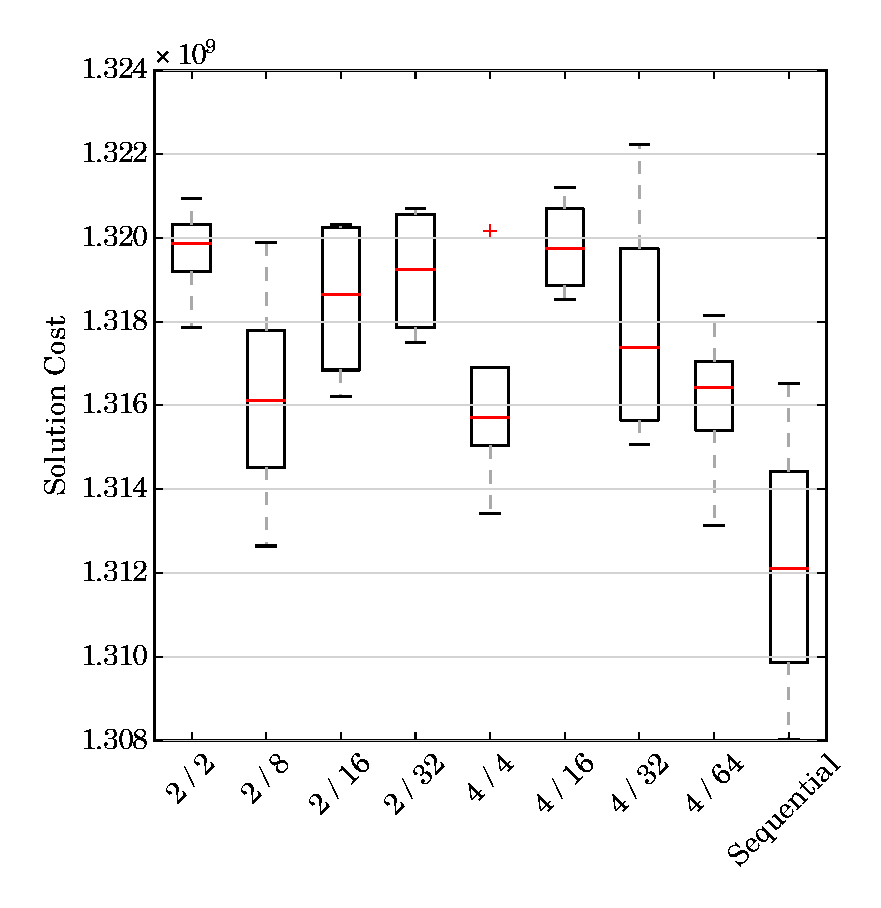
\includegraphics[scale=.48]{pla85900_15min_boxplot}
        \caption{Boxplots of 4 runs solving an instance of size 85900 with
                 different numbers of VMs and requests per VM.}
        \label{fig:85900boxplot}
    \end{minipage}%
    \hfill
    \begin{minipage}{.48\textwidth}
        \centering
        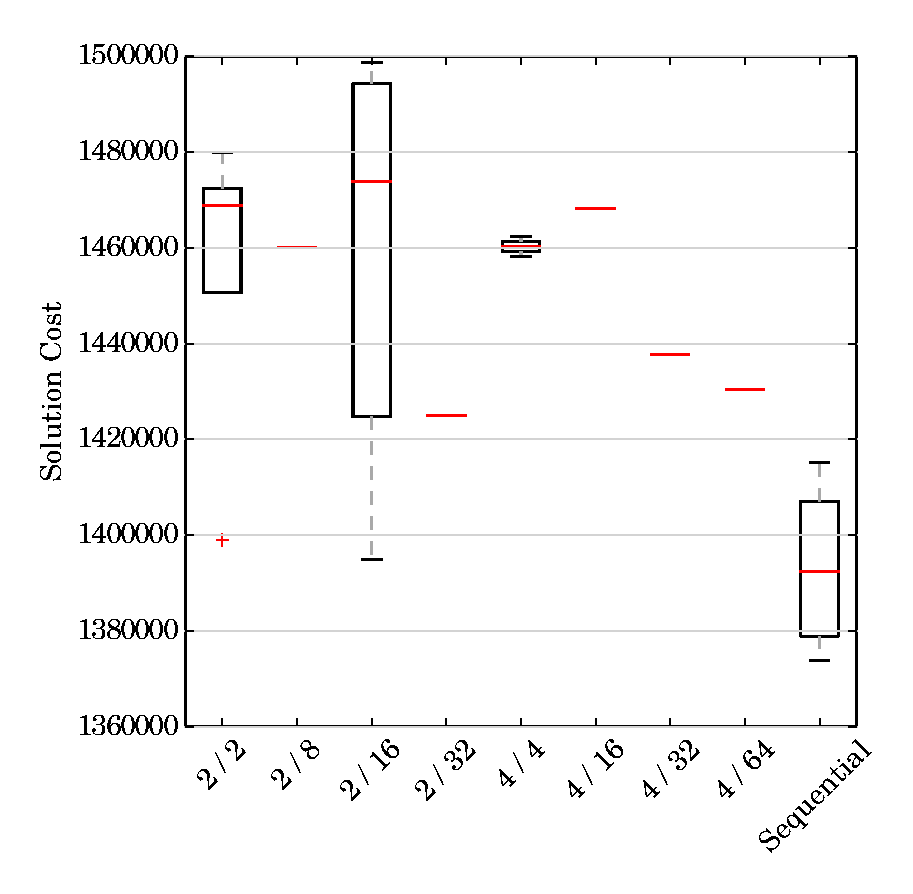
\includegraphics[scale=.48]{att532_15min_boxplot}
        \caption{Boxplots of 4 runs solving an instance of size 532 with
                 different numbers of VMs and requests per VM.}
        \label{fig:532boxplot}
    \end{minipage}%
    \label{fig:boxplots}
\end{figure}

Figures~\ref{fig:532tspi2} and~\ref{fig:532tspi4} show the best runs in the
instance of size 532 for the unmodified OpenTuner and for each VM
configuration.  Figures~\ref{fig:85900tspi2} and~\ref{fig:85900tspi4} show the
same measurements for the instance of size 85900.  The time overhead in
relation to the unmodified OpenTuner is clearly visible in
Figures~\ref{fig:532tspi2} to~\ref{fig:85900tspi4}, and is due to the
initialization of the cloud application.

\begin{figure}[htpb]
    \centering
    \begin{minipage}{.48\textwidth}
        \centering
        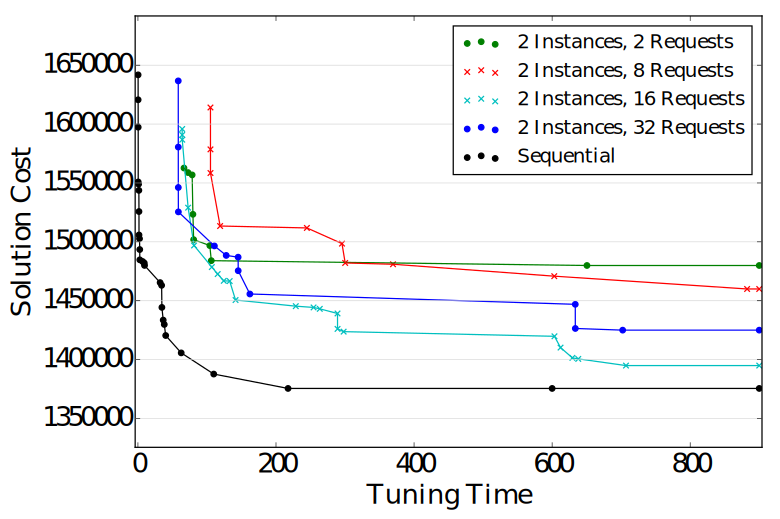
\includegraphics[scale=.43]{i2_p_n_comparison}
        \caption{Measurements using two VM instances, solving
                 a TSP instance of size 532.}
        \label{fig:532tspi2}
    \end{minipage}%
    \hfill
    \begin{minipage}{.48\textwidth}
        \centering
        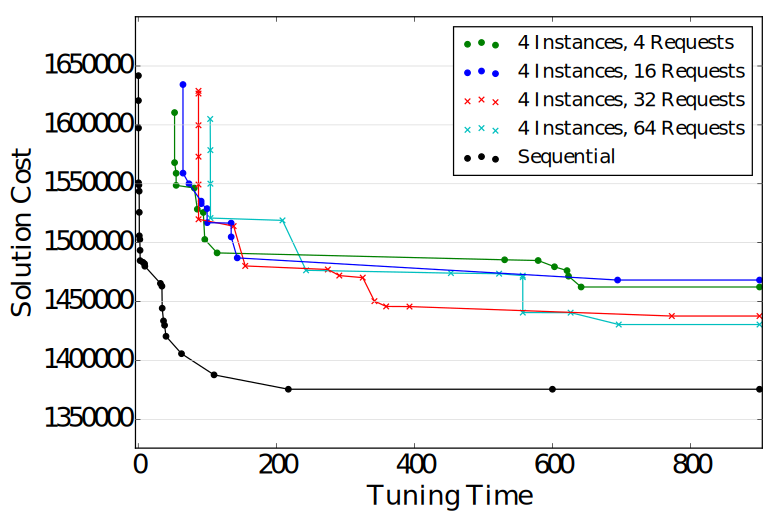
\includegraphics[scale=.43]{i4_p_n_comparison}
        \caption{Measurements using four VM instances,
                 solving a TSP instance of size 532.}
        \label{fig:532tspi4}
    \end{minipage}%
    \label{fig:532tsp}
\end{figure}

The tuning runs using our methodology and protocol depend on the initialization
of a cloud application, and start to produce results later in the tuning run.
Despite the graphs from figures~\ref{fig:532tspi2} to~\ref{fig:85900tspi4} show
that the solution costs of the results obtained with our methodology are worst
than the ones obtained with the unmodified OpenTuner, the cost of running the
same VM instance used in our experiments with the Google Compute Engine were as
low as
US\$0.038~\footnote{\path{cloud.google.com/compute/pricing#predefined_machine_types}
[Accessed on 23 December 2015]} per hour, per instance. The financial cost of
obtaining an autotuned solution of a given quality with our methodology is
therefore considerably lower than the financial cost of acquiring a machine
capable of finding the same solution. This is the main advantage of our
proposal.

\begin{figure}[htpb]
    \centering
    \begin{minipage}{.48\textwidth}
        \centering
        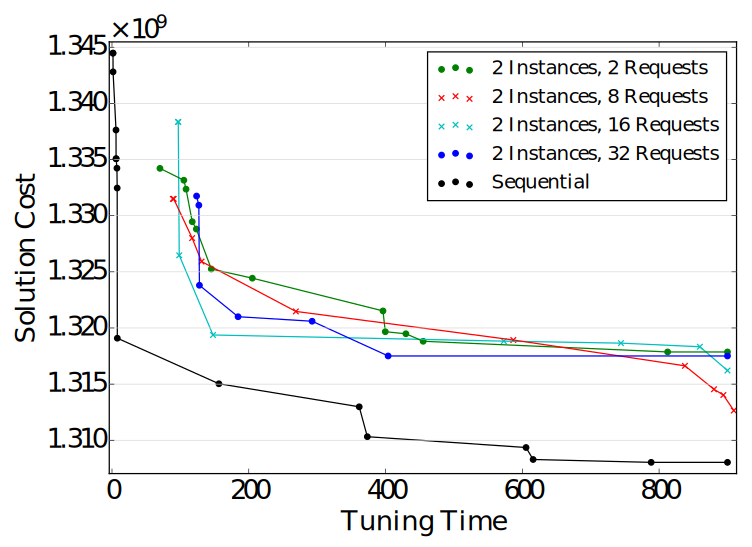
\includegraphics[scale=.35]{i2_p_n_comparison_85900}
        \caption{Measurements using two VM instances,
                 solving an instance of size 85900.}
        \label{fig:85900tspi2}
    \end{minipage}%
    \hfill
    \begin{minipage}{.48\textwidth}
        \centering
        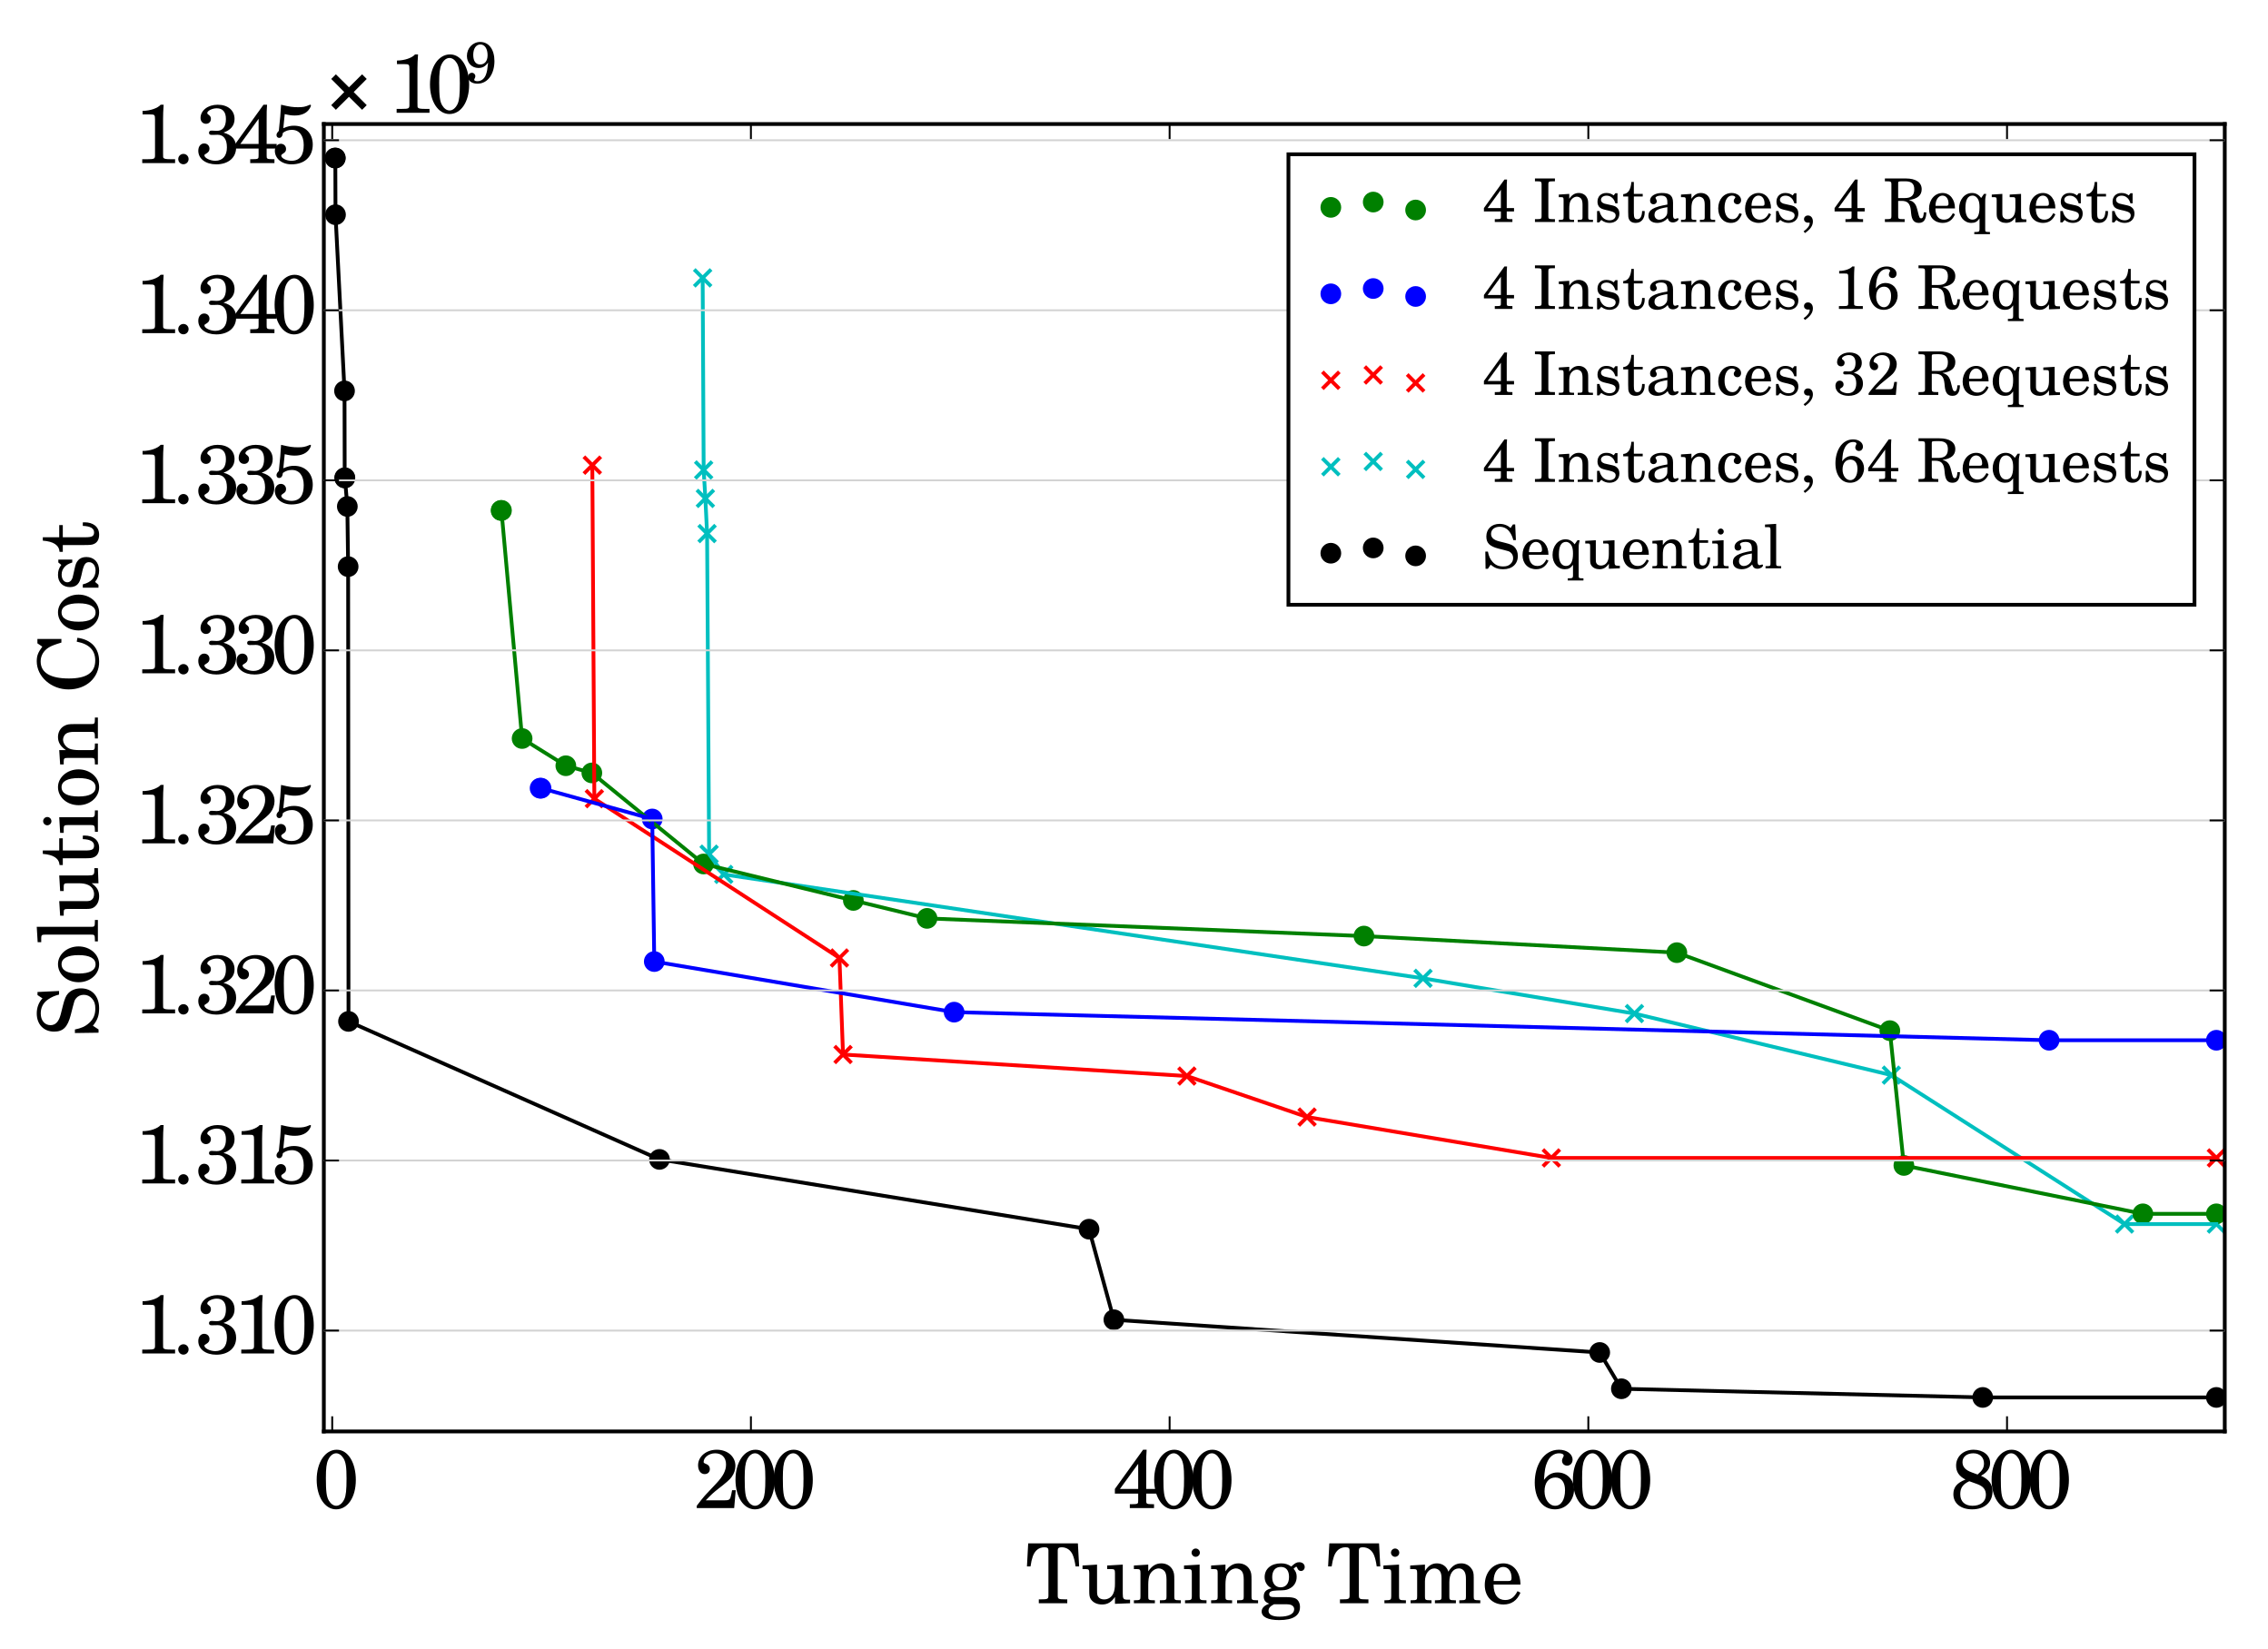
\includegraphics[scale=.35]{i4_p_n_comparison_85900}
        \caption{Measurements using four VM instances,
                 solving an instance of size 85900.}
        \label{fig:85900tspi4}
    \end{minipage}%
    \label{fig:85900tsp}
\end{figure}

\subsection{Summary and Future Work}
\label{sec:cloud-conclusion}

Future work will analyze the performance of our methodology and protocol in
different problem domains, determining the ones that benefit the most from this
approach. To effectively leverage cloud computing for autotuning it will be
necessary to better understand how VM initialization, communication and tuning
times impact performance. We would like to run more extensive experiments and
use different public clouds.

We will also study normalization techniques, composing benchmarks of problems
that expose architecture-dependant features to the autotuner and analyzing the
performance of our proposed techniques in those problems.
